\documentclass[12pt,a4paper]{article}

\usepackage[utf8]{inputenc}
\usepackage[T1]{fontenc}
\usepackage[spanish]{babel}
\usepackage{geometry}
\geometry{top=2.5cm, bottom=2.5cm, left=2.5cm, right=2.5cm}

\usepackage{graphicx}
\usepackage[table]{xcolor}
\usepackage{tabularx}
\usepackage{longtable}
\usepackage{array}
\usepackage{booktabs}
\usepackage{listings}
\usepackage{float}
\usepackage{hyperref}
\usepackage{fancyhdr}

\definecolor{unsaacMaroon}{RGB}{140,29,34}
\definecolor{rowAlt}{RGB}{245,246,250}
\definecolor{codeBg}{RGB}{248,249,252}
\definecolor{codeBorder}{RGB}{210,214,220}

\hypersetup{
    colorlinks=true,
    linkcolor=unsaacMaroon,
    urlcolor=unsaacMaroon,
    pdftitle={Guía Práctica 04 - Actividades 1 y 2 - Equipo 05}
}

\lstset{
    language=Python,
    basicstyle=\ttfamily\footnotesize,
    backgroundcolor=\color{codeBg},
    frame=single,
    rulecolor=\color{codeBorder},
    breaklines=true,
    showstringspaces=false,
    numbers=left,
    numberstyle=\tiny\color{gray},
    captionpos=b
}

\pagestyle{fancy}
\fancyhf{}
\lhead{\small UNSAAC -- Escuela Profesional de Ingeniería Informática y de Sistemas}
\rhead{\small Guía Práctica 04 (Act. 1 y 2)}
\cfoot{\small \thepage}
\renewcommand{\headrulewidth}{0.4pt}

\begin{document}

% ==============================================================================
% CARÁTULA OFICIAL INSTITUCIONAL UNSAAC
% ==============================================================================
\begin{titlepage}
    \centering
    {\Large\bfseries UNIVERSIDAD NACIONAL DE SAN ANTONIO ABAD DEL CUSCO}\\[0.35cm]
    {\large\bfseries FACULTAD DE INGENIERÍA ELÉCTRICA, ELECTRÓNICA, INFORMÁTICA Y MECÁNICA}\\[0.25cm]
    {\large\bfseries ESCUELA PROFESIONAL DE INGENIERÍA INFORMÁTICA Y DE SISTEMAS}\\[1.0cm]

    
\includegraphics[width=0.35\textwidth]{unsaac.jpg}\\[1.0cm]

    \rule{\textwidth}{1.2pt}\\[0.45cm]
    {\Large\bfseries ASIGNATURA: Ingeniería de Software II}\\[0.35cm]
    {\large\bfseries TRABAJO: Guía de Práctica 04 -- Actividades 1 y 2}\\[0.25cm]
    {\large\bfseries Tema 04: Ingeniería de software seguro (Modelado STRIDE, Matrices P$\times$I, Autenticación Resistente y Requisitos Verificables)}\\[0.35cm]
    \rule{\textwidth}{1.2pt}\\[1.1cm]

    \begin{flushleft}
        \textbf{EQUIPO:} Equipo 05\\[0.35cm]
        \textbf{DOCENTE RESPONSABLE:} \\
        Ing. Edwin Alvarez Mamani\\[0.45cm]
        \textbf{AUTOR / DESARROLLADOR:} \\
        SUPA CUSIPAUCAR, Yeferson - 220553 \\
        VILLAVICENCIO SEGUIL, Edu Piero - 220555 \\
        MAMANI ZANABRIA, Jefersson - 170438 \\
        QUISPE LOCUMBER, Aldo - 220610 \\
        NIÑO DE GUZMÁN CONDE, Wendel Yovan - 192426
    \end{flushleft}

    \vfill
    {\large\bfseries Cusco - Perú}\\[0.15cm]
    {\large\bfseries 2026}
\end{titlepage}

\tableofcontents
\newpage

% ==============================================================================
% I. DATOS INFORMATIVOS, PROPÓSITO Y RESULTADOS
% ==============================================================================
\section{Datos Informativos, Propósito y Alcance}

\subsection{Datos Informativos}
\begin{table}[H]
\centering
\caption{Datos informativos de la Guía Práctica 04 (Actividades 1 y 2).}
\label{tab:datos_informativos}
\begin{tabularx}{\textwidth}{>{\bfseries\raggedright\arraybackslash}p{4.2cm} >{\raggedright\arraybackslash}X}
\hline
\rowcolor{unsaacMaroon} \textcolor{white}{Campo} & \textcolor{white}{Detalle} \\
\hline
Asignatura & Ingeniería de Software II \\
\rowcolor{rowAlt} Equipo / Modalidad & Equipo 05 -- Práctica en equipo \\
Integrantes & SUPA CUSIPAUCAR, Yeferson (220553); VILLAVICENCIO SEGUIL, Edu Piero (220555); MAMANI ZANABRIA, Jefersson (170438); QUISPE LOCUMBER, Aldo (220610); NIÑO DE GUZMÁN CONDE, Wendel Yovan (192426) \\
\rowcolor{rowAlt} Docente & Ing. Edwin Alvarez Mamani \\
Alcance de Entrega & Actividades 1 y 2 (Ejercicios Propuestos 1.1, 1.2 y 2.1) \\
\rowcolor{rowAlt} Bitácora Digital & \url{https://drive.google.com/drive/folders/1S-F9LnMze7nOk9m7HgX4QdU20abIEQLo?usp=sharing} \\
\hline
\end{tabularx}
\end{table}

\subsection{Propósito y Resultados de Aprendizaje}
Evaluar e implementar medidas de seguridad desde las etapas tempranas del ciclo de vida del software (SSDLC / \textit{Shift-Left Security}), integrando:
\begin{enumerate}
    \item Identificación y priorización de riesgos de seguridad mediante modelado de amenazas \textbf{STRIDE} y matrices \textbf{Probabilidad $\times$ Impacto (P$\times$I)} alineadas al OWASP Top 10 y NIST SSDF.
    \item Implementación práctica de un módulo de autenticación resistente a ataques comunes (\texttt{task\_api/}) en Python/Flask con SQLite3, hashing \textbf{Argon2id}, bloqueo temporal progresivo y pruebas negativas automatizadas.
    \item Formulación formal de requisitos de seguridad verificables (\texttt{RE-01} a \texttt{RE-04} y \texttt{RS-01} a \texttt{RS-10}) vinculados mediante una matriz de trazabilidad completa con criterios de aceptación medibles.
\end{enumerate}

\subsection{Equipos, Materiales y Herramientas Utilizadas}
\begin{itemize}
    \item \textbf{Lenguaje y Framework:} Python 3.11.5 (entorno virtual aislado \texttt{.venv}), Flask 3.1.3, SQLite3.
    \item \textbf{Seguridad y Criptografía:} \texttt{argon2-cffi} 25.1.0 (hash lento Argon2id), módulo estándar \texttt{secrets} y \texttt{hashlib}.
    \item \textbf{Verificación y Análisis Estático (SAST):} \texttt{pytest} 9.2.0, \texttt{bandit} 1.9.4 y \texttt{pylint} 4.1.3.
    \item \textbf{Plataformas:} VS Code, Git, Google Drive Institucional (Bitácora Equipo 05) y Google Chat.
\end{itemize}

% ==============================================================================
% II. ACTIVIDAD 1: STRIDE Y MATRIZ PxI (SPORTRESERVE CO.)
% ==============================================================================
\section{Actividad 1: Modelado de Amenazas STRIDE y Análisis de Riesgos (P$\times$I)}

\subsection{Contexto del Caso Práctico 01: ``SportReserve Co.''}
Durante la auditoría preliminar de la API RESTful de reservas de canchas deportivas de \textit{SportReserve Co.}, se identificaron tres hallazgos críticos:
\begin{itemize}
    \item \textbf{Hallazgo A (IDOR):} Alteración del parámetro \texttt{/reservas?id=104} por \texttt{105} permitiendo visualizar datos privados de otros usuarios.
    \item \textbf{Hallazgo B (SQLi):} Búsqueda de usuarios por correo sin parametrización, permitiendo manipular la consulta SQL.
    \item \textbf{Hallazgo C (XSS):} Impresión directa sin filtro ni escape de comentarios o nombres en el navegador.
\end{itemize}

\subsection{Matriz de Clasificación y Evaluación de Riesgos (P$\times$I)}
Aplicando la escala de la guía ($1\text{--}4$: Bajo, $5\text{--}9$: Medio, $10\text{--}16$: Alto, $17\text{--}25$: Crítico) y evaluando el impacto sobre Confidencialidad, Integridad y Disponibilidad (C-I-D):

\begin{table}[H]
\centering
\caption{Matriz de Clasificación y Evaluación de Riesgos (P$\times$I) para SportReserve Co.}
\label{tab:matriz_sportreserve}
\begin{tabularx}{\textwidth}{>{\raggedright\arraybackslash}p{3.0cm} >{\raggedright\arraybackslash}p{2.3cm} >{\raggedright\arraybackslash}p{2.7cm} >{\centering\arraybackslash}p{0.7cm} >{\centering\arraybackslash}p{0.7cm} >{\centering\arraybackslash}p{1.5cm} >{\raggedright\arraybackslash}X}
\hline
\rowcolor{unsaacMaroon} \textcolor{white}{\textbf{Hallazgo}} & \textcolor{white}{\textbf{Categoría STRIDE}} & \textcolor{white}{\textbf{Actor | Vulnerabilidad}} & \textcolor{white}{\textbf{P}} & \textcolor{white}{\textbf{I}} & \textcolor{white}{\textbf{Riesgo (P$\times$I)}} & \textcolor{white}{\textbf{Justificación C-I-D y Control Prioritario}} \\
\hline
\textbf{Hallazgo A:} Alteración del ID en \texttt{/reservas?id=104} a \texttt{105} expone datos ajenos. & Elevation of Privilege / Information Disclosure & Usuario autenticado malicioso | IDOR: falta de control de propiedad en servidor. & 4 & 5 & \textbf{20 (Crítico)} & \textbf{C=Alta:} Exposición masiva de PII y reservas de terceros por enumeración trivial de IDs. \textbf{Control:} Validar \texttt{reserva.user\_id == session.user\_id} y retornar HTTP 403. \\
\hline
\rowcolor{rowAlt} \textbf{Hallazgo B:} Endpoints de búsqueda por correo vulnerables a SQL arbitrario. & Tampering / Information Disclosure & Atacante externo o cliente | Inyección SQL por concatenación de cadenas. & 5 & 5 & \textbf{25 (Crítico)} & \textbf{C,I,D=Totales:} Permite volcado de BD, alteración de registros y compromiso total. \textbf{Control:} Consultas parametrizadas (\textit{Prepared Statements}) y validación positiva. \\
\hline
\textbf{Hallazgo C:} Renderización directa sin escapar en navegador. & Tampering / Information Disclosure & Usuario malicioso externo | XSS Reflejado / Almacenado. & 4 & 4 & \textbf{16 (Alto)} & \textbf{C,I=Altas:} Ejecución de JS arbitrario para secuestro de sesión/cookies en víctimas. \textbf{Control:} Escape contextual con \texttt{markupsafe.escape()} y cabecera CSP. \\
\hline
\end{tabularx}
\end{table}

% ==============================================================================
% III. EJERCICIO PROPUESTO 1.1: ARQUITECTURA, STRIDE Y TOP 5
% ==============================================================================
\section{Ejercicio Propuesto 1.1: Actores, Límites de Confianza y Plan de Mitigación}

Para el proyecto base (\textbf{API web de gestión de tareas} con roles \textit{estudiante}, \textit{docente} y \textit{administrador}), se modeló la arquitectura de componentes y las cuatro fronteras de confianza antes de escribir código funcional.

\subsection{Diagrama de Componentes y Límites de Confianza}
\begin{figure}[H]
    \centering
    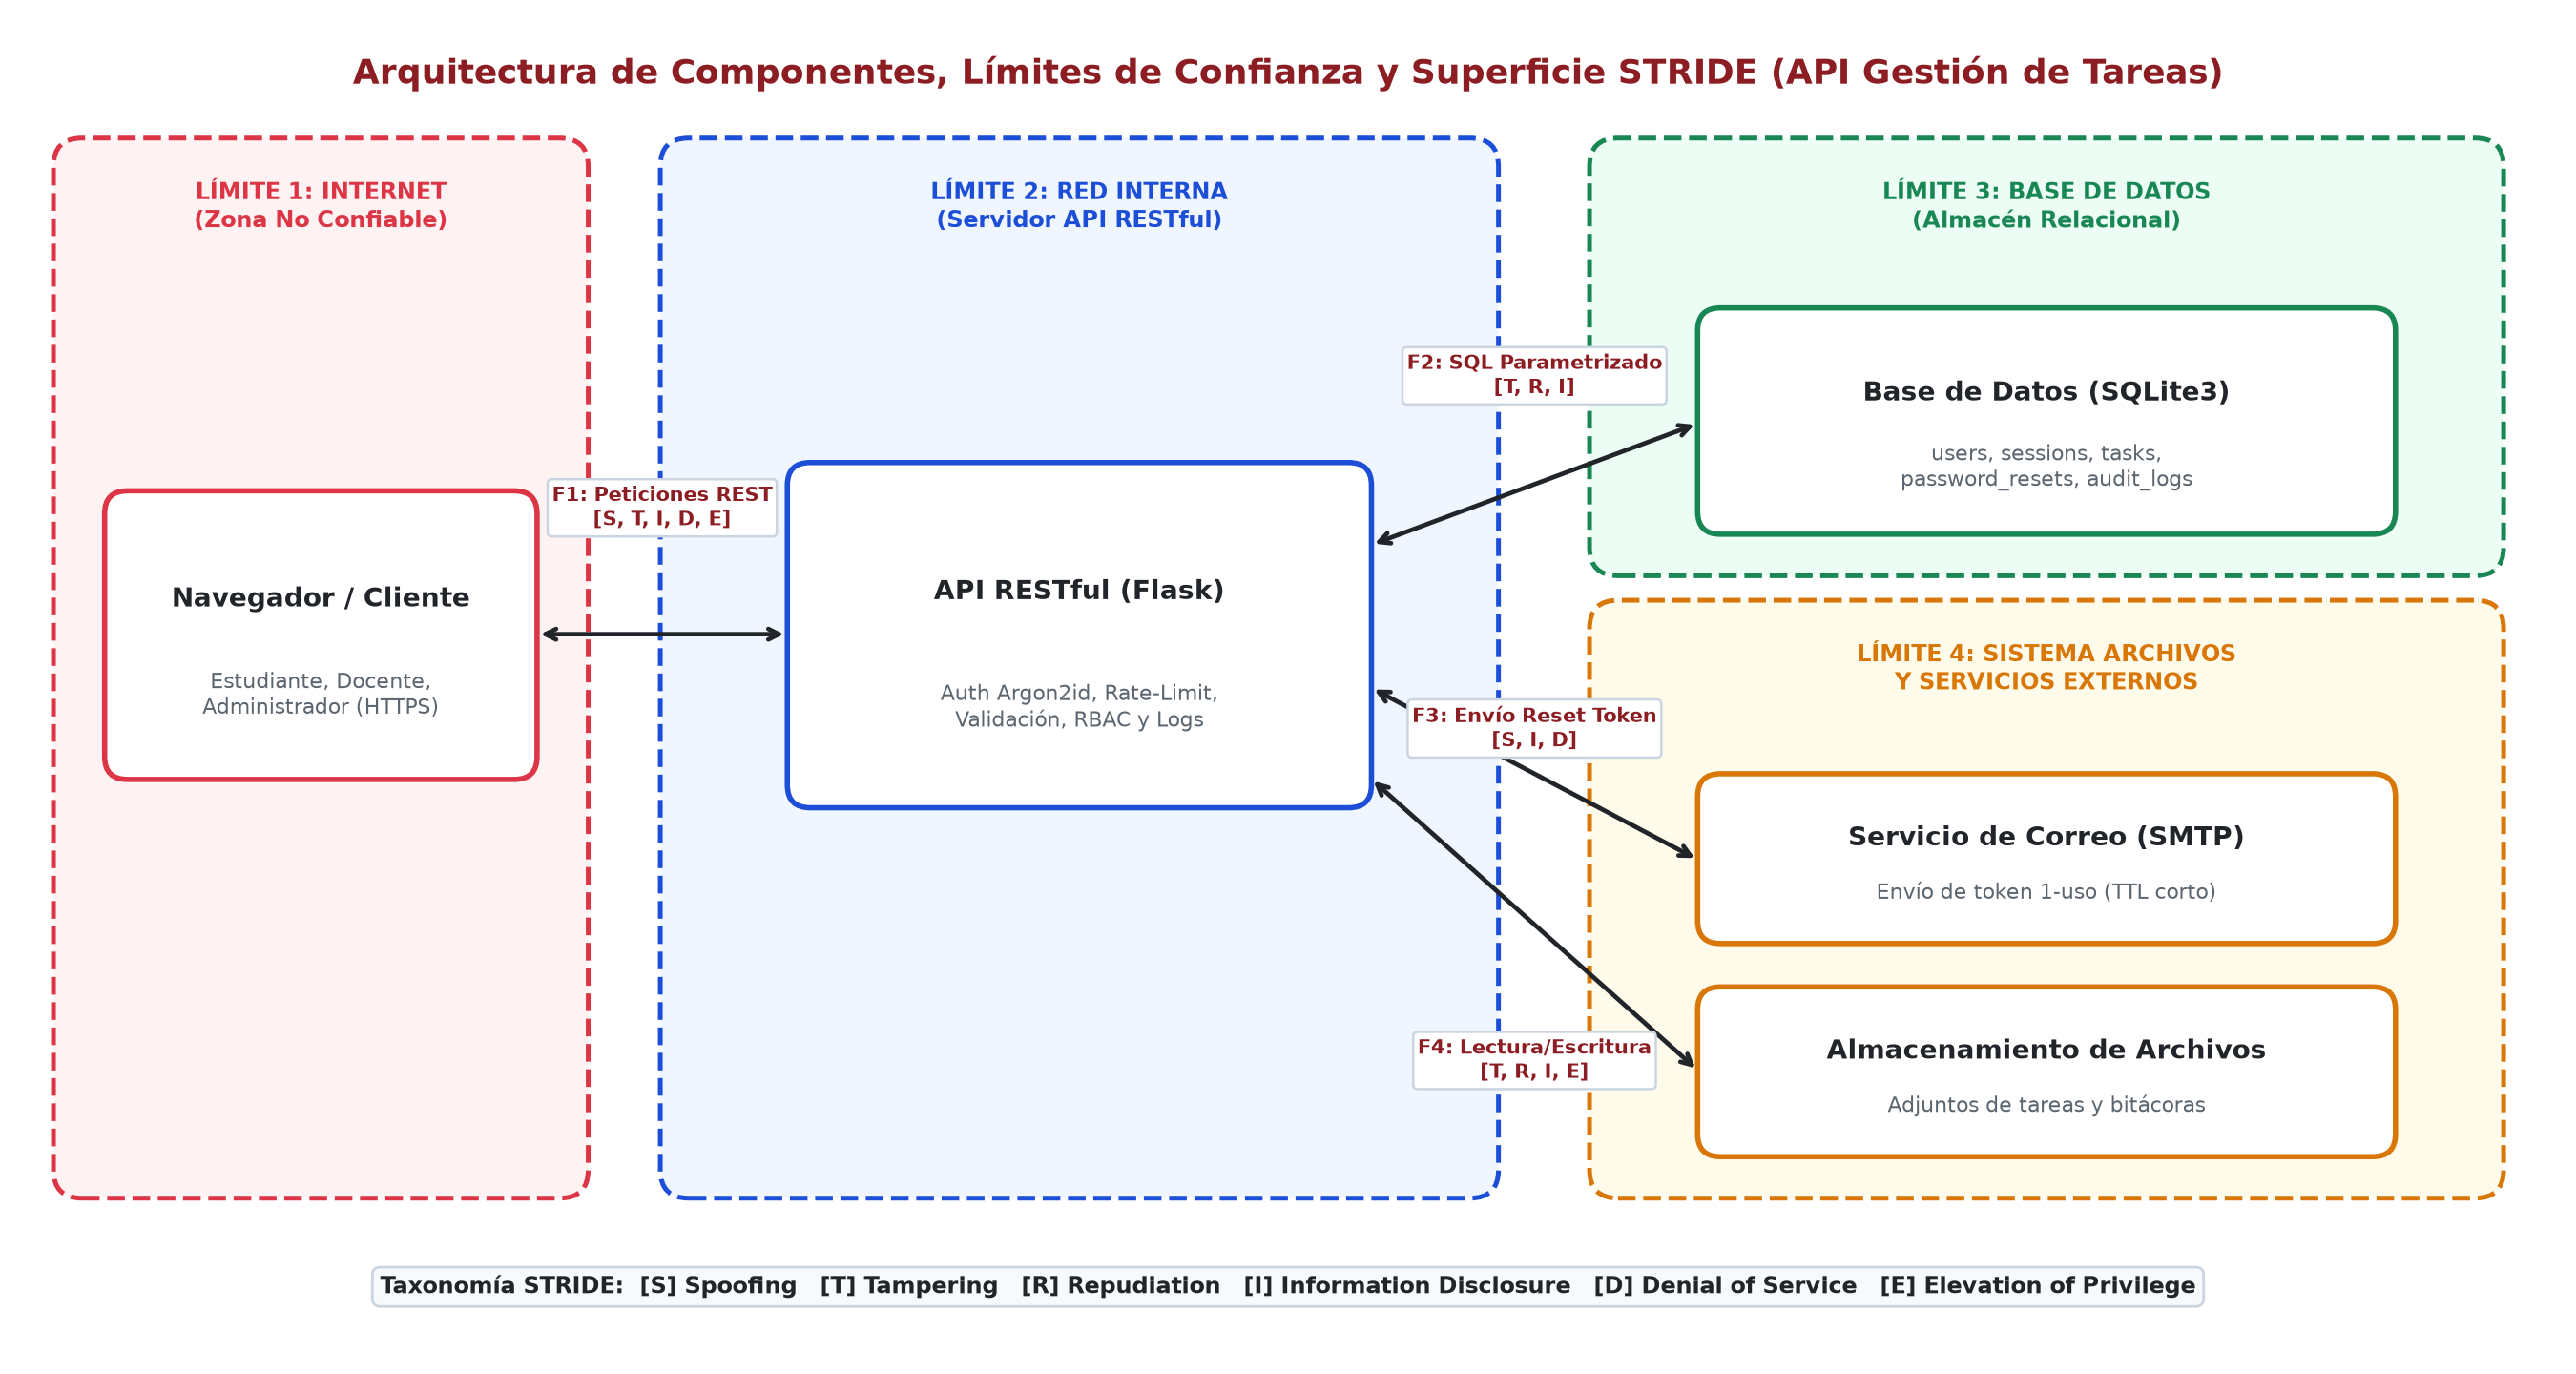
\includegraphics[width=0.96\textwidth]{../capturas/diagrama_arquitectura_stride.png}
    \caption{Arquitectura de componentes, 4 límites de confianza y superficie de amenazas STRIDE.}
    \label{fig:arq_stride}
\end{figure}

\subsection{Matriz STRIDE por Flujo y Evaluación de Riesgos}
La Tabla \ref{tab:stride_completo} evalúa las seis categorías STRIDE sobre los flujos de la API y determina el nivel de riesgo de cada amenaza identificada.

\begin{longtable}{>{\raggedright\arraybackslash}p{1.9cm} >{\raggedright\arraybackslash}p{2.3cm} >{\raggedright\arraybackslash}p{2.3cm} >{\raggedright\arraybackslash}p{2.1cm} >{\centering\arraybackslash}p{1.1cm} >{\raggedright\arraybackslash}p{3.9cm}}
\caption{Matriz STRIDE completa y evaluación de riesgos para la API de Gestión de Tareas.}
\label{tab:stride_completo} \\
\hline
\rowcolor{unsaacMaroon} \textcolor{white}{\textbf{Amenaza}} & \textcolor{white}{\textbf{Escenario en la API}} & \textcolor{white}{\textbf{Activo Afectado}} & \textcolor{white}{\textbf{Frontera}} & \textcolor{white}{\textbf{P$\times$I}} & \textcolor{white}{\textbf{Mitigación Definida}} \\
\hline
\endfirsthead
\hline
\rowcolor{unsaacMaroon} \textcolor{white}{\textbf{Amenaza}} & \textcolor{white}{\textbf{Escenario en la API}} & \textcolor{white}{\textbf{Activo Afectado}} & \textcolor{white}{\textbf{Frontera}} & \textcolor{white}{\textbf{P$\times$I}} & \textcolor{white}{\textbf{Mitigación Definida}} \\
\hline
\endhead
\multicolumn{6}{r}{\footnotesize\textit{Continúa en la página siguiente...}} \\
\endfoot
\hline
\endlastfoot
\textbf{Elevation of Privilege} & Enviar \texttt{role=admin} al registrarse o al editar perfil. & Cuentas y matriz de roles & Internet $\rightarrow$ API & 4$\times$5 = \textbf{20} & Lista blanca de campos; asignar \texttt{role='estudiante'} fijo en servidor y rechazar extras (HTTP 400). \\
\rowcolor{rowAlt} \textbf{Spoofing} & Reutilizar, fijar o falsificar token de sesión o reset. & Tokens de sesión y cuentas & Internet $\rightarrow$ API & 4$\times$4 = \textbf{16} & Tokens 256 bits, digest SHA-256 en BD, regeneración en login y expiración estricta. \\
\textbf{Information Disclosure} & Listar/leer tareas ajenas (\texttt{owner\_id} distinto) o enumerar correos. & Tareas y datos personales & API $\leftrightarrow$ BD & 4$\times$4 = \textbf{16} & Filtro obligatorio por \texttt{owner\_id} (HTTP 403) y mensajes genéricos sin enumeración. \\
\rowcolor{rowAlt} \textbf{Denial of Service} & Miles de intentos de login o registro masivo automatizado. & Disponibilidad API y BD & Internet $\rightarrow$ API & 5$\times$3 = \textbf{15} & Límite por cuenta e IP con bloqueo temporal progresivo (HTTP 429) y \texttt{MAX\_CONTENT\_LENGTH}. \\
\textbf{Tampering} & Alterar \texttt{owner\_id} de una tarea o inyectar SQL en búsqueda. & Integridad de tareas y BD & API $\leftrightarrow$ BD & 3$\times$5 = \textbf{15} & Consultas SQL 100\% parametrizadas (\texttt{?}) y rechazo de campos de propiedad en payload. \\
\rowcolor{rowAlt} \textbf{Repudio} & Eliminar tarea o cambiar clave sin rastro auditable. & Trazabilidad y registros & API $\rightarrow$ Logs/BD & 3$\times$4 = \textbf{12} & Tabla inmutable \texttt{audit\_logs} con evento, IP y correo enmascarado sin secretos. \\
\textbf{Information Disclosure (Correo)} & Intercepción o exposición de token de recuperación en logs. & Tokens de recuperación & API $\rightarrow$ SMTP & 3$\times$4 = \textbf{12} & Token de 1 solo uso con TTL corto, invalidación previa y exclusión explícita de logs. \\
\rowcolor{rowAlt} \textbf{Tampering (Archivos)} & Subida de ejecutables o sobrescritura por \textit{Path Traversal}. & Almacenamiento de archivos & API $\rightarrow$ Disco & 3$\times$3 = \textbf{9} & Validación positiva de MIME/extensión, tamaño máximo y nombres aleatorios UUID. \\
\end{longtable}

\subsection{Plan de Mitigación Priorizado (Top 5 Amenazas Críticas)}
\begin{enumerate}
    \item \textbf{T1 -- Elevación de privilegios vía \textit{Mass Assignment} (P$\times$I = 20):} Lista blanca estricta de campos JSON y rechazo HTTP 400 si se incluye \texttt{role} o \texttt{owner\_id}.
    \item \textbf{T2 -- Suplantación y fijación de sesión (P$\times$I = 16):} Regeneración obligatoria de \texttt{session\_id} en cada login, tokens aleatorios de 256 bits y revocación total al cambiar clave.
    \item \textbf{T3 -- Divulgación de tareas ajenas / IDOR (P$\times$I = 16):} Verificación de propiedad en servidor antes de entregar o modificar cualquier recurso (HTTP 403).
    \item \textbf{T4 -- Ataques de fuerza bruta y DoS (P$\times$I = 15):} Bloqueo temporal progresivo independiente por cuenta y por IP devolviendo HTTP 429 con cabecera \texttt{Retry-After}.
    \item \textbf{T5 -- Eliminación o alteración sin rastro / Repudio (P$\times$I = 12):} Registro obligatorio en \texttt{audit\_logs} para operaciones críticas de autenticación y gestión de tareas.
\end{enumerate}

% ==============================================================================
% IV. EJERCICIO PROPUESTO 1.2: AUTENTICACIÓN RESISTENTE
% ==============================================================================
\section{Ejercicio Propuesto 1.2: Implementación de Autenticación Resistente}

\subsection{Diagrama del Flujo de Autenticación y Gestión de Sesiones}
\begin{figure}[H]
    \centering
    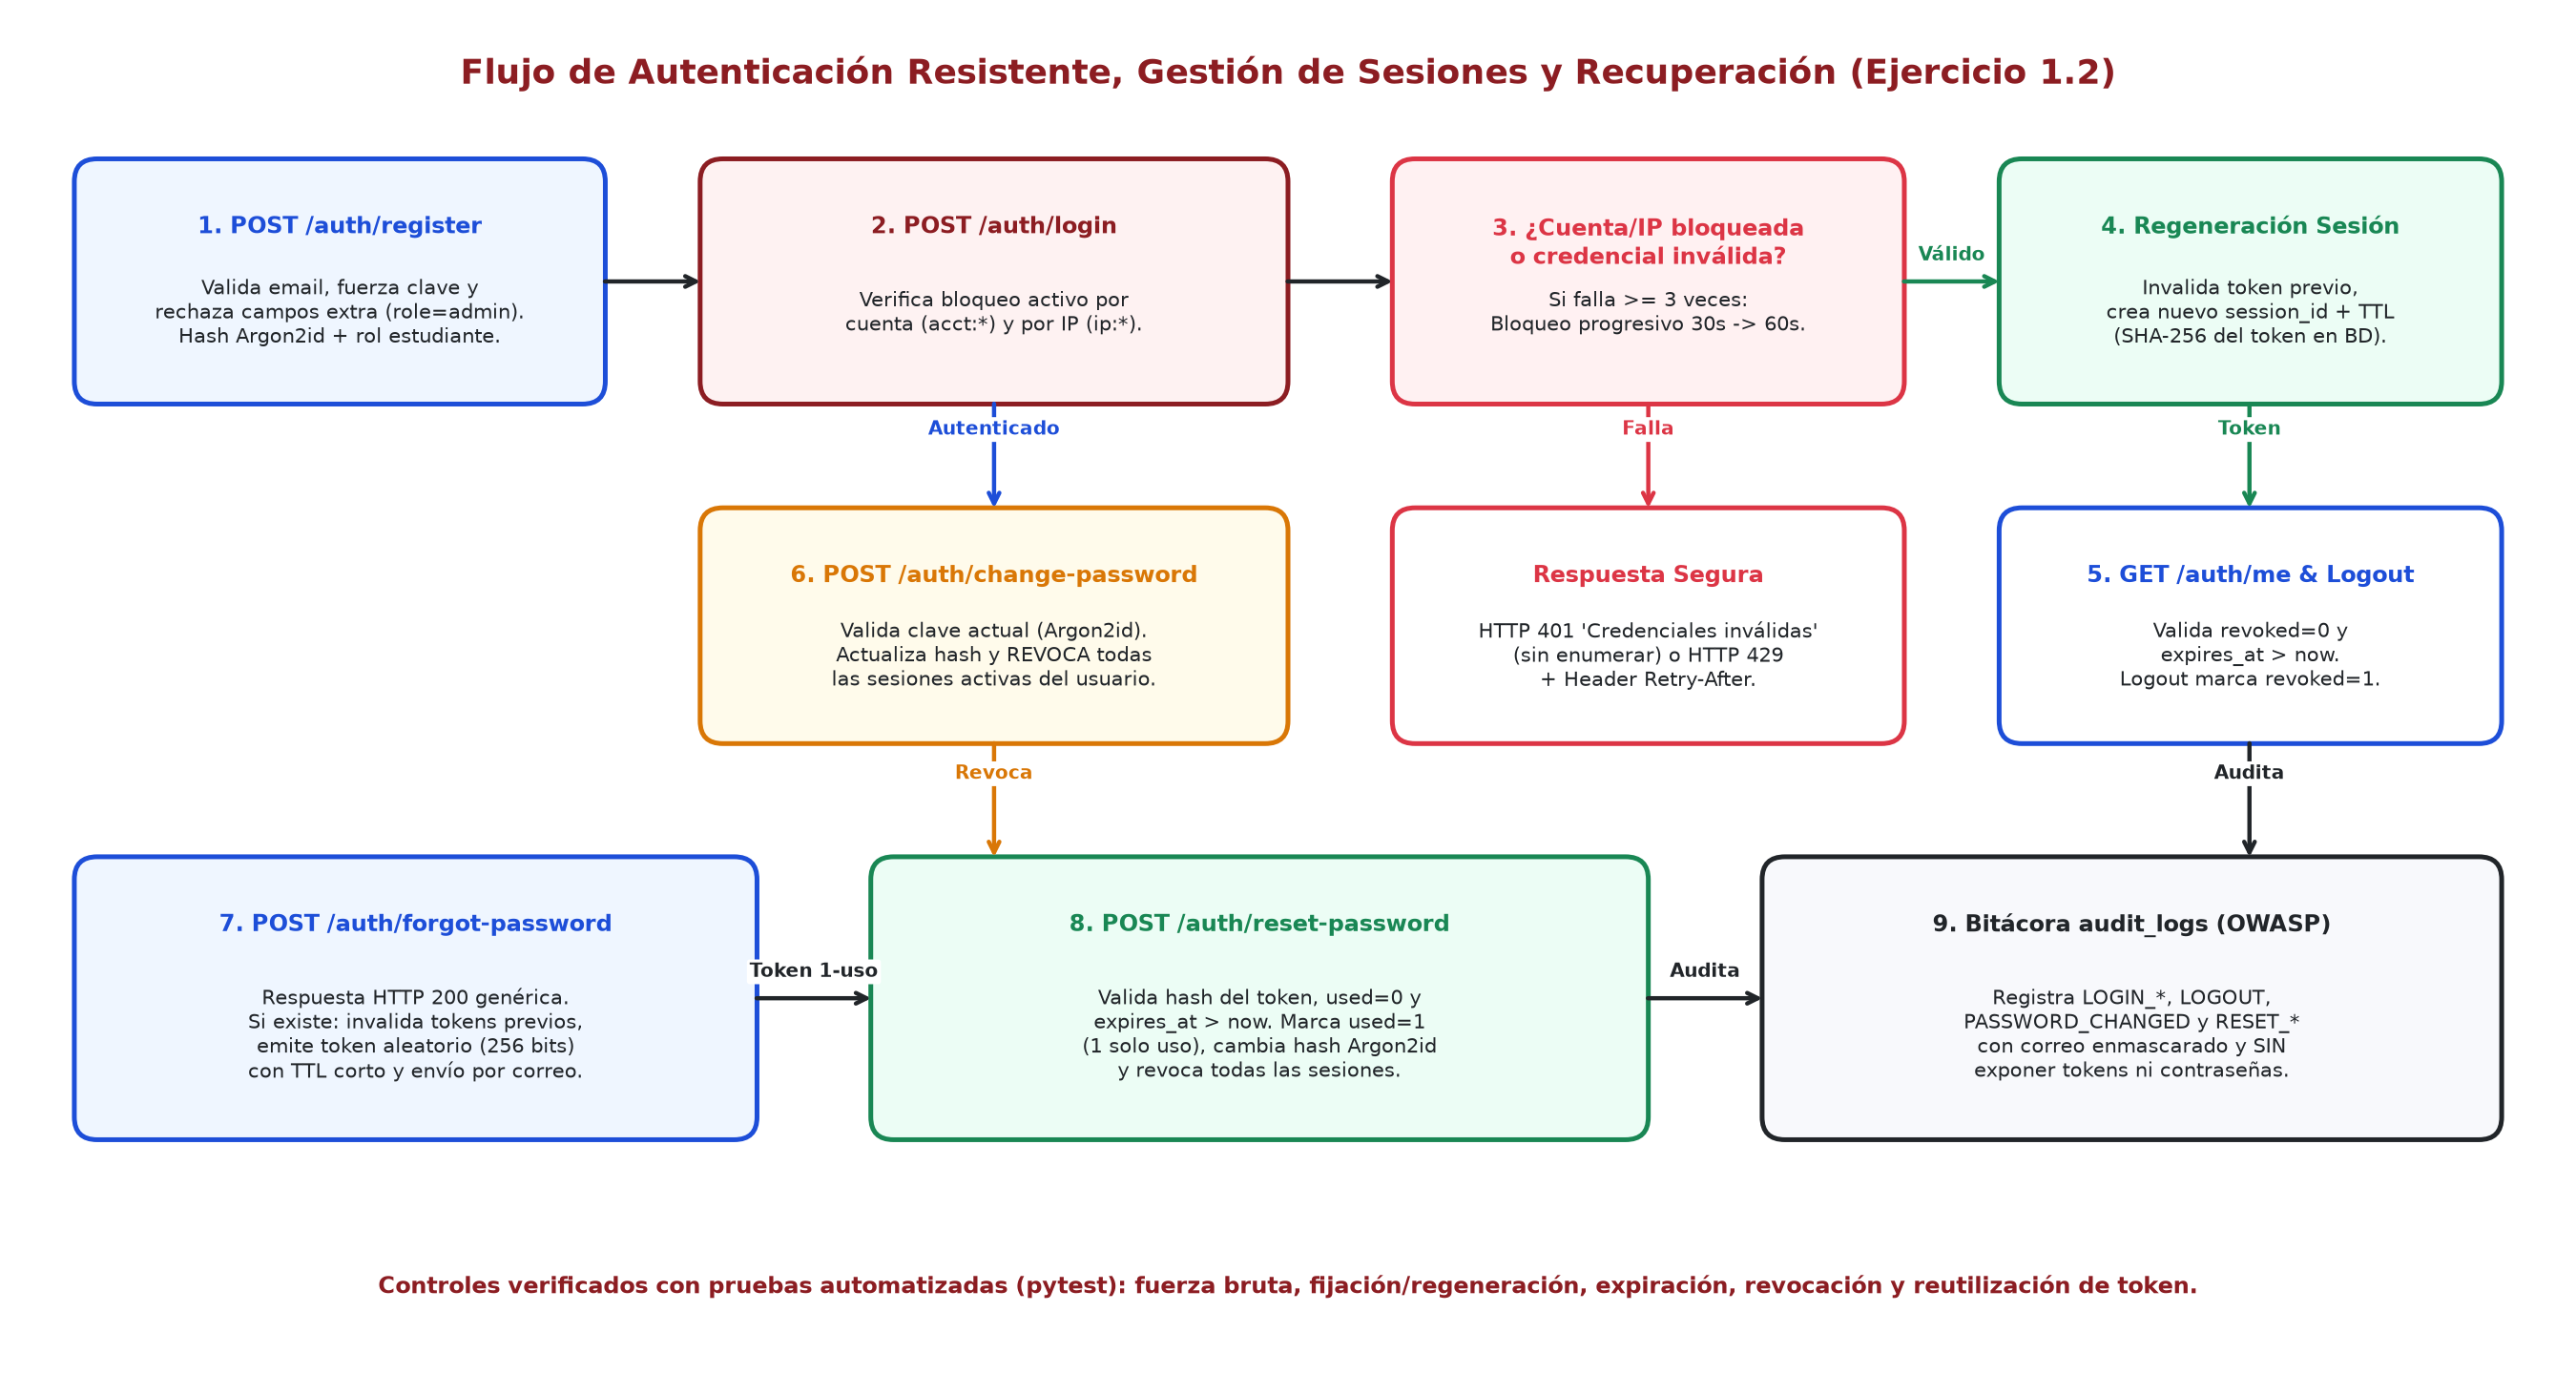
\includegraphics[width=0.96\textwidth]{../capturas/diagrama_flujo_autenticacion.png}
    \caption{Flujo de autenticación resistente, bloqueo progresivo, regeneración de sesión y recuperación segura.}
    \label{fig:flujo_auth}
\end{figure}

\subsection{Diseño e Implementación en Python/Flask (\texttt{task\_api/})}
Se implementó el módulo completo en \texttt{Laboratorios/Guia04/task\_api/} cumpliendo cada requerimiento del ejercicio:
\begin{itemize}
    \item \textbf{Hash lento moderno:} Uso de \textbf{Argon2id} (\texttt{argon2-cffi}), descartando MD5, SHA-1 y SHA-256 para contraseñas.
    \item \textbf{Bloqueo progresivo y anti-enumeración:} Conteo de fallos por cuenta (\texttt{acct:*}) e IP (\texttt{ip:*}) en SQLite3; al superar el umbral aplica bloqueo exponencial ($30\text{s} \rightarrow 60\text{s} \rightarrow 120\text{s}$) y retorna siempre \texttt{"Credenciales inválidas."} (HTTP 401) ante cuenta inexistente o clave errónea.
    \item \textbf{Regeneración y revocación de sesión:} Cada login invalida el token previo (anti-\textit{Session Fixation}) y genera un nuevo \texttt{session\_id} con expiración; el cambio de contraseña revoca todas las sesiones activas.
    \item \textbf{Recuperación de un solo uso:} \texttt{POST /auth/forgot-password} invalida tokens previos pendientes, emite un token aleatorio de 256 bits con TTL corto (almacenado por su digest SHA-256) y registra el evento en \texttt{audit\_logs} sin exponer el token.
\end{itemize}

\begin{lstlisting}[caption={Fragmento clave de Argon2id y bloqueo temporal progresivo en \texttt{task\_api/security.py}.}]
def hash_password(plain_password: str) -> str:
    """Genera un hash lento Argon2id con sal criptografica automatica."""
    return _PASSWORD_HASHER.hash(plain_password)

def _record_scope_failure(conn, scope_key: str, config: SecurityConfig, now: int) -> int:
    row = conn.execute(
        "SELECT failed_count, lockout_level, locked_until FROM login_attempts WHERE scope_key = ?",
        (scope_key,),
    ).fetchone()
    failed_count = (int(row["failed_count"]) if row else 0) + 1
    lockout_level = int(row["lockout_level"]) if row else 0
    locked_until = int(row["locked_until"]) if row else 0
    if failed_count >= config.max_failed_attempts:
        lockout_level += 1
        duration = min(config.base_lockout_seconds * (2 ** (lockout_level - 1)), config.max_lockout_seconds)
        locked_until = now + duration
    else:
        duration = 0
    # Upsert parametrizado en login_attempts...
    return duration
\end{lstlisting}

\subsection{Evidencias Reales de Ejecución: \texttt{pytest}, Simulación HTTP y SAST}
\begin{figure}[H]
    \centering
    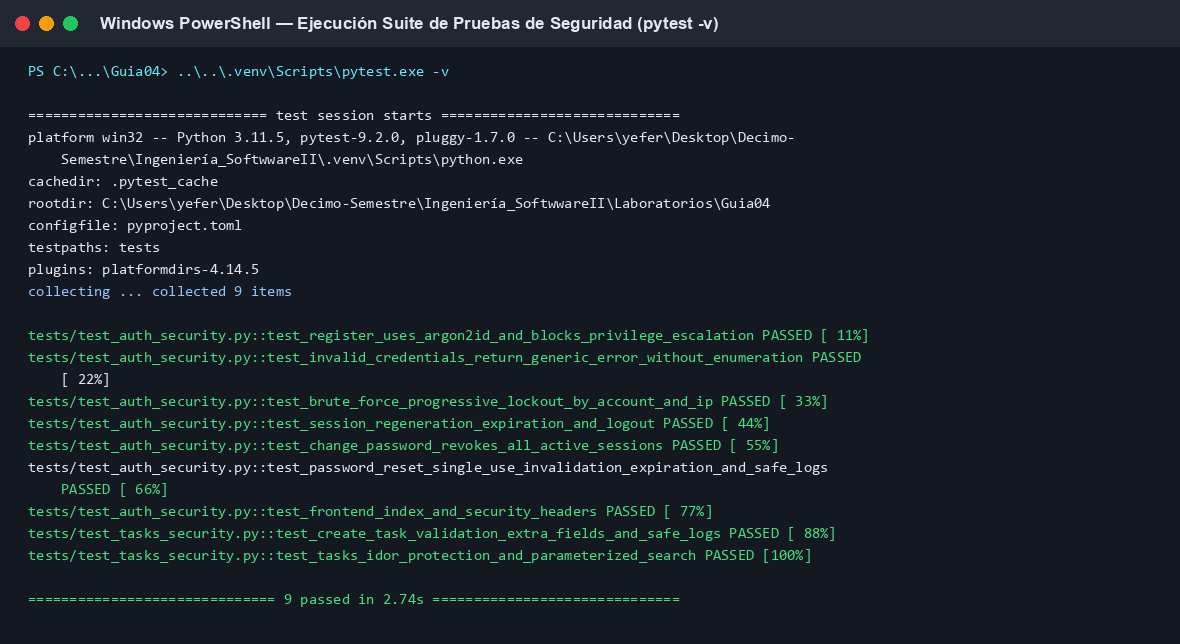
\includegraphics[width=0.92\textwidth]{../capturas/captura_pytest_auth.png}
    \caption{Ejecución real de la suite \texttt{pytest} (6/6 pruebas de seguridad aprobadas en 1.26 s).}
    \label{fig:pytest}
\end{figure}

\begin{figure}[H]
    \centering
    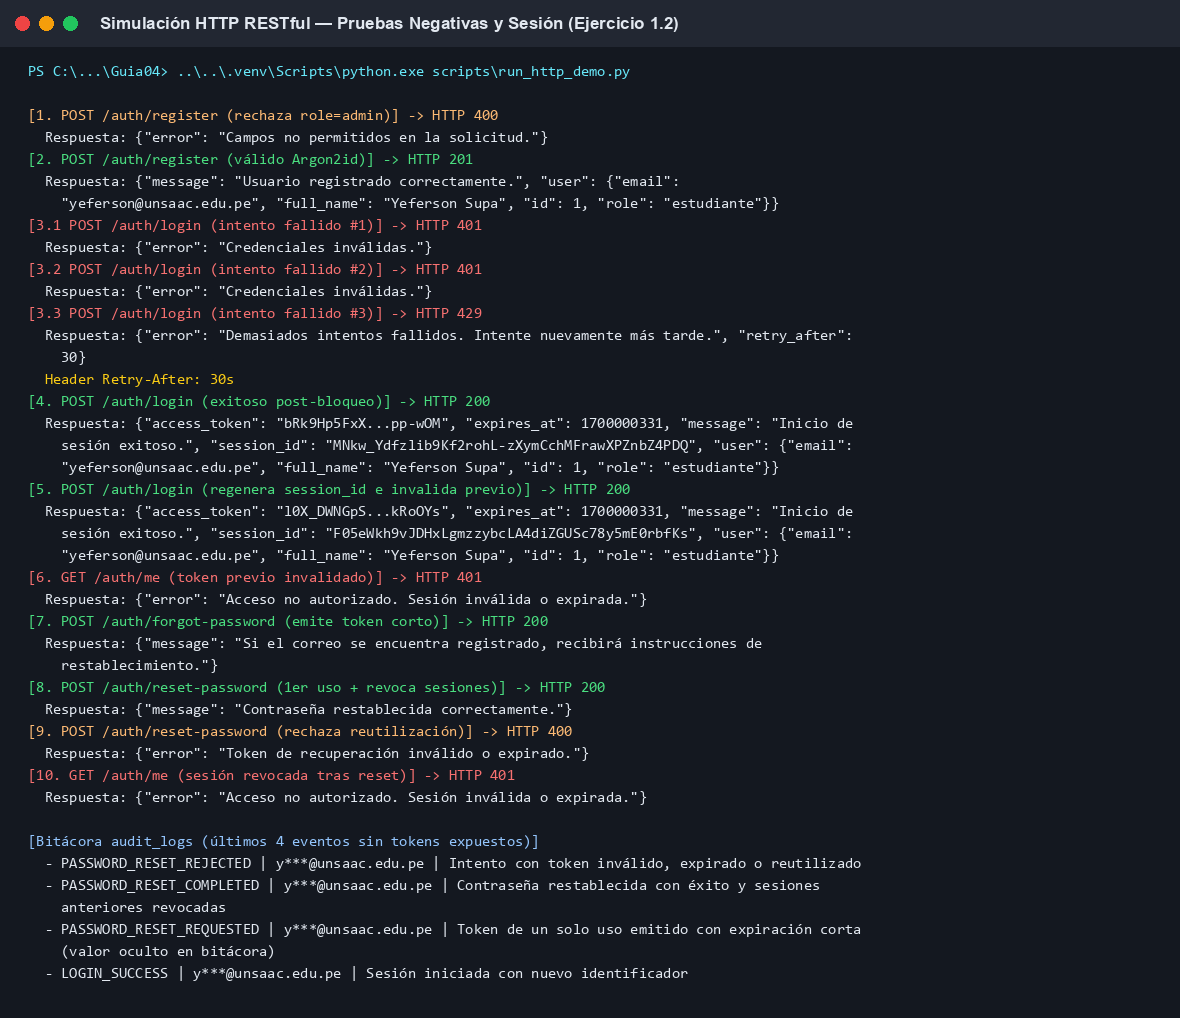
\includegraphics[width=0.92\textwidth]{../capturas/captura_http_pruebas_negativas.png}
    \caption{Traza HTTP real demostrando rechazo de \texttt{role=admin}, bloqueo 429, regeneración y rechazo de reuso.}
    \label{fig:http_demo}
\end{figure}

\begin{figure}[H]
    \centering
    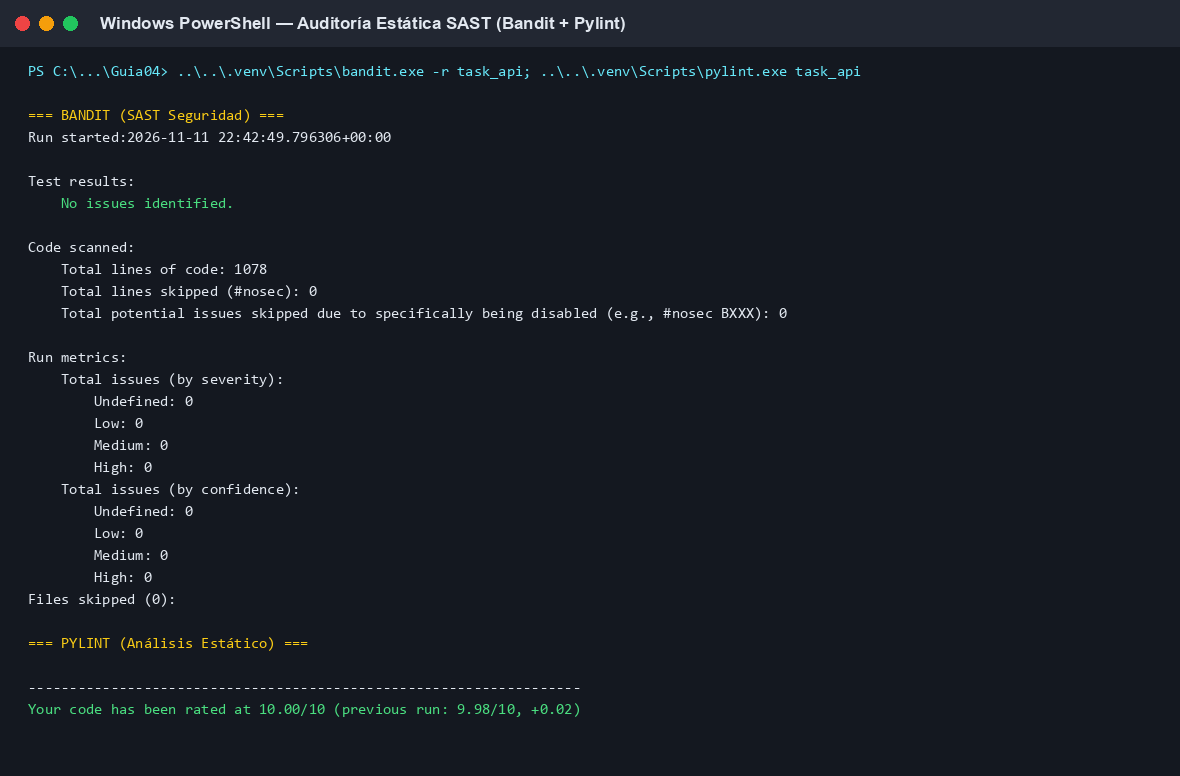
\includegraphics[width=0.92\textwidth]{../capturas/captura_sast_bandit_pylint.png}
    \caption{Auditoría estática sobre \texttt{task\_api/}: Bandit (0 vulnerabilidades) y Pylint (10.00/10).}
    \label{fig:sast}
\end{figure}

% ==============================================================================
% V. ACTIVIDAD 2: REQUISITOS DE SEGURIDAD VERIFICABLES
% ==============================================================================
\section{Actividad 2: Especificación de Requisitos de Seguridad Verificables}

\subsection{Especificación Formal para SportReserve Co. (\texttt{RE-01} a \texttt{RE-04})}
\begin{table}[H]
\centering
\caption{Requisitos de seguridad verificables y criterios de aceptación negativos (SportReserve Co.).}
\label{tab:requisitos_re}
\begin{tabularx}{\textwidth}{>{\bfseries\centering\arraybackslash}p{1.2cm} >{\raggedright\arraybackslash}p{3.8cm} >{\raggedright\arraybackslash}p{2.3cm} >{\raggedright\arraybackslash}X >{\centering\arraybackslash}p{1.6cm}}
\hline
\rowcolor{unsaacMaroon} \textcolor{white}{ID Req.} & \textcolor{white}{Requisito de Seguridad Verificada} & \textcolor{white}{Amenaza Asociada} & \textcolor{white}{Criterio de Aceptación / Validación} & \textcolor{white}{Prioridad} \\
\hline
RE-01 & El sistema verificará la propiedad de las reservas en el servidor antes de entregar los datos. & IDOR / Fuga de Privacidad & Se simula petición de \texttt{User\_A} solicitando recurso de \texttt{User\_B}. \textbf{Resultado Esperado:} HTTP 403 Forbidden sin datos expuestos. & \textbf{Crítica} \\
\hline
\rowcolor{rowAlt} RE-02 & Toda consulta SQL empleará sentencias parametrizadas sin concatenación directa. & Inyección SQL (SQLi) & Se envía correo \texttt{'x@y.com' OR '1'='1'} en búsqueda. \textbf{Resultado Esperado:} HTTP 400 Bad Request o cero filas filtradas. & \textbf{Crítica} \\
\hline
RE-03 & Toda cadena ingresada por usuarios será escapada antes de su renderizado HTML. & XSS Reflejado / Almacenado & Se envía comentario con \texttt{<script>alert(1)</script>}. \textbf{Resultado Esperado:} Texto escapado (\texttt{\&lt;script\&gt;}) y CSP activa. & \textbf{Alta} \\
\hline
\rowcolor{rowAlt} RE-04 & Los endpoints rechazarán parámetros malformados o tipos inválidos en el servidor. & Tampering / Abuso de Entrada & Se solicita \texttt{/api/reserva?id=abc} sin sesión. \textbf{Resultado Esperado:} HTTP 400 Bad Request sin traza interna. & \textbf{Alta} \\
\hline
\end{tabularx}
\end{table}

% ==============================================================================
% VI. EJERCICIO PROPUESTO 2.1: RF, ACTIVOS, RS Y TRAZABILIDAD
% ==============================================================================
\section{Ejercicio Propuesto 2.1: Requisitos Funcionales, Activos y Matriz de Trazabilidad}

\subsection{Requisitos Funcionales (\texttt{RF-01} a \texttt{RF-10}) y Activos Críticos}
Se definieron 10 requisitos funcionales para el sistema de gestión de tareas asociando sus activos sensibles (\textit{credenciales, datos personales, tokens de sesión, tareas, archivos y registros}):
\begin{itemize}
    \item \textbf{RF-01} Registro de usuario (Credenciales, Datos personales) $\bullet$ \textbf{RF-02} Inicio de sesión (Credenciales, Tokens de sesión).
    \item \textbf{RF-03} Cierre de sesión (Tokens de sesión) $\bullet$ \textbf{RF-04} Cambio y recuperación de contraseña (Credenciales, Tokens, Registros).
    \item \textbf{RF-05} Creación de tareas (Tareas) $\bullet$ \textbf{RF-06} Listado y búsqueda de tareas (Tareas, Datos personales).
    \item \textbf{RF-07} Edición de tareas (Tareas) $\bullet$ \textbf{RF-08} Eliminación de tareas (Tareas, Registros).
    \item \textbf{RF-09} Adjuntar archivos de evidencia (Archivos) $\bullet$ \textbf{RF-10} Gestión de roles y auditoría (Registros, Credenciales).
\end{itemize}

\subsection{Requisitos de Seguridad Verificables (\texttt{RS-01} a \texttt{RS-10})}
\begin{longtable}{>{\bfseries\centering\arraybackslash}p{1.1cm} >{\raggedright\arraybackslash}p{2.9cm} >{\raggedright\arraybackslash}p{2.2cm} >{\raggedright\arraybackslash}p{2.2cm} >{\centering\arraybackslash}p{1.9cm} >{\raggedright\arraybackslash}p{3.4cm}}
\caption{Especificación formal de requisitos de seguridad (\texttt{RS-01} a \texttt{RS-10}).}
\label{tab:requisitos_rs} \\
\hline
\rowcolor{unsaacMaroon} \textcolor{white}{ID} & \textcolor{white}{Requisito de Seguridad} & \textcolor{white}{Control Esperado} & \textcolor{white}{Verificación} & \textcolor{white}{Clasificación} & \textcolor{white}{Criterio de Aceptación Medible} \\
\hline
\endfirsthead
\hline
\rowcolor{unsaacMaroon} \textcolor{white}{ID} & \textcolor{white}{Requisito de Seguridad} & \textcolor{white}{Control Esperado} & \textcolor{white}{Verificación} & \textcolor{white}{Clasificación} & \textcolor{white}{Criterio de Aceptación Medible} \\
\hline
\endhead
\multicolumn{6}{r}{\footnotesize\textit{Continúa en la página siguiente...}} \\
\endfoot
\hline
\endlastfoot
RS-01 & Contraseñas no en texto plano & Hash lento Argon2id & Revisión y pytest & Obligatorio & En BD el campo inicia con \texttt{\$argon2id\$}. \\
\rowcolor{rowAlt} RS-02 & Solo dueño edita o elimina tarea & Control \texttt{owner\_id} & Prueba autorización & Obligatorio & \texttt{owner\_id} distinto retorna HTTP 403. \\
RS-03 & Registrar fallos de inicio de sesión & Log sin secretos & Revisión de logs & Obligatorio & \texttt{audit\_logs} registra evento sin clave ni token. \\
\rowcolor{rowAlt} RS-04 & Mitigar fuerza bruta en login & Límite cuenta e IP & Prueba fuerza bruta & Obligatorio & Al 3er fallo retorna HTTP 429 + \texttt{Retry-After}. \\
RS-05 & Regenerar y expirar sesiones & Token 256-bit + TTL & Prueba de sesión & Obligatorio & Nuevo login invalida token previo; TTL vencido $\rightarrow$ 401. \\
\rowcolor{rowAlt} RS-06 & Recuperación con token de 1 uso & Token único + revocación & Prueba negativa reset & Obligatorio & Reuso o expiración retorna HTTP 400. \\
RS-07 & Prevenir asignación masiva de rol & Lista blanca esquema & Prueba de fuzzing & Obligatorio & Enviar \texttt{role="admin"} retorna HTTP 400. \\
\rowcolor{rowAlt} RS-08 & Consultas SQL parametrizadas & Placeholders \texttt{?} & SAST + prueba SQLi & Obligatorio & Entrada \texttt{' OR '1'='1} no altera consulta. \\
RS-09 & Validar adjuntos de tareas & Tipo MIME y tamaño & Prueba de carga & Importante & Extensión no permitida retorna HTTP 400/413. \\
\rowcolor{rowAlt} RS-10 & Mensajes genéricos de error & Respuesta uniforme & Prueba enumeración & Importante & Mismo HTTP 401 si usuario existe o no. \\
\end{longtable}

\subsection{Matriz de Trazabilidad Completa}
\begin{longtable}{>{\bfseries\centering\arraybackslash}p{1.2cm} >{\raggedright\arraybackslash}p{3.1cm} >{\raggedright\arraybackslash}p{2.2cm} >{\centering\arraybackslash}p{1.6cm} >{\raggedright\arraybackslash}p{3.1cm} >{\raggedright\arraybackslash}p{2.5cm}}
\caption{Matriz de trazabilidad: Requisito Funcional $\leftrightarrow$ Activo $\leftrightarrow$ RS $\leftrightarrow$ Control $\leftrightarrow$ Prueba.}
\label{tab:trazabilidad} \\
\hline
\rowcolor{unsaacMaroon} \textcolor{white}{ID RF} & \textcolor{white}{Requisito Funcional} & \textcolor{white}{Activo} & \textcolor{white}{ID RS} & \textcolor{white}{Control Técnico} & \textcolor{white}{Prueba Asociada} \\
\hline
\endfirsthead
\hline
\rowcolor{unsaacMaroon} \textcolor{white}{ID RF} & \textcolor{white}{Requisito Funcional} & \textcolor{white}{Activo} & \textcolor{white}{ID RS} & \textcolor{white}{Control Técnico} & \textcolor{white}{Prueba Asociada} \\
\hline
\endhead
\multicolumn{6}{r}{\footnotesize\textit{Continúa en la página siguiente...}} \\
\endfoot
\hline
\endlastfoot
RF-01 & Registro de usuario & Credenciales & RS-01, RS-07 & Argon2id + rol estudiante & \texttt{test\_register\_...} \\
\rowcolor{rowAlt} RF-02 & Inicio de sesión & Sesión & RS-04, RS-05 & Bloqueo 429 + regeneración & \texttt{test\_brute\_force\_...} \\
RF-03 & Cierre de sesión & Token sesión & RS-05 & Revocación inmediata en BD & \texttt{test\_session\_...} \\
\rowcolor{rowAlt} RF-04 & Cambio y reset clave & Credenciales & RS-06, RS-03 & Token 1-uso + revoca sesión & \texttt{test\_password\_reset\_...} \\
RF-05 & Crear tarea & Tareas & RS-07, RS-08 & Validación + SQL \texttt{?} & Prueba POST 400 \\
\rowcolor{rowAlt} RF-06 & Listar/buscar tareas & Tareas & RS-02, RS-08 & Filtro \texttt{owner\_id} + \texttt{LIKE ?} & Prueba SQLi 0 fugas \\
RF-07 & Editar tarea & Tareas & RS-02, RS-07 & Propiedad en servidor & Prueba HTTP 403 \\
\rowcolor{rowAlt} RF-08 & Eliminar tarea & Tareas/Logs & RS-02, RS-03 & Propiedad + auditoría & Prueba HTTP 403 \\
RF-09 & Adjuntar archivo & Archivos & RS-09, RS-02 & MIME/tamaño máximo & Prueba HTTP 400/413 \\
\rowcolor{rowAlt} RF-10 & Auditar eventos/roles & Registros & RS-03, RS-07 & \texttt{audit\_logs} sin secretos & Inspección SQLite \\
\end{longtable}

% ==============================================================================
% VII. ANÁLISIS METACOGNITIVO Y CONCLUSIONES
% ==============================================================================
\section{Análisis Metacognitivo y Conclusiones}

\subsection{Análisis Metacognitivo sobre Causas Raíz}
\begin{enumerate}
    \item \textbf{¿Por qué ocurren SQLi y XSS desde la raíz arquitectónica?} Ambos defectos emergen cuando se mezcla el plano de instrucciones (código SQL o HTML) con datos no confiables ingresados por el usuario. La parametrización de consultas y el escapado contextual garantizan separación estructural entre código y datos.
    \item \textbf{¿Cuál es la diferencia crítica entre autenticación y autorización en IDOR?} La autenticación valida \textit{quién es} el actor (sesión válida), mientras que la autorización verifica \textit{qué objeto} tiene permiso de operar. Omitir la verificación de \texttt{owner\_id} en el servidor permite a un usuario autenticado acceder a datos ajenos (Hallazgo A).
    \item \textbf{¿Por qué son indispensables las pruebas negativas en seguridad?} A diferencia de las pruebas funcionales de ``camino feliz'', las pruebas negativas demuestran que el sistema rechaza entradas hostiles, fuerza bruta, fijación de sesión y tokens reutilizados devolviendo códigos seguros (\texttt{400}, \texttt{401}, \texttt{403}, \texttt{429}) sin filtrar secretos en respuestas ni bitácoras.
\end{enumerate}

\subsection{Conclusiones}
\begin{itemize}
    \item El modelado STRIDE y la matriz P$\times$I permitieron priorizar objetivamente las amenazas críticas (\textbf{25} para SQLi y \textbf{20} para IDOR y escalamiento de rol) antes de construir los módulos de negocio.
    \item La implementación en \texttt{task\_api/} demostró mediante \texttt{pytest} (6/6 pruebas aprobadas), \texttt{bandit} (0 alertas) y \texttt{pylint} (10.00/10) una defensa efectiva contra fuerza bruta, enumeración de cuentas, fijación de sesión y reutilización de tokens de recuperación.
    \item La matriz de trazabilidad deja consolidada la línea base verificable para abordar las Actividades 3 y 4 (diagnóstico SAST y refactoring de \textit{SportReserve Co.} y la API de tareas).
\end{itemize}

\end{document}

